\input{preamble.tex}
\begin{document}
\def\title{Universidad de Guadalajara - Los Mismísimos Carajillos}
\centering{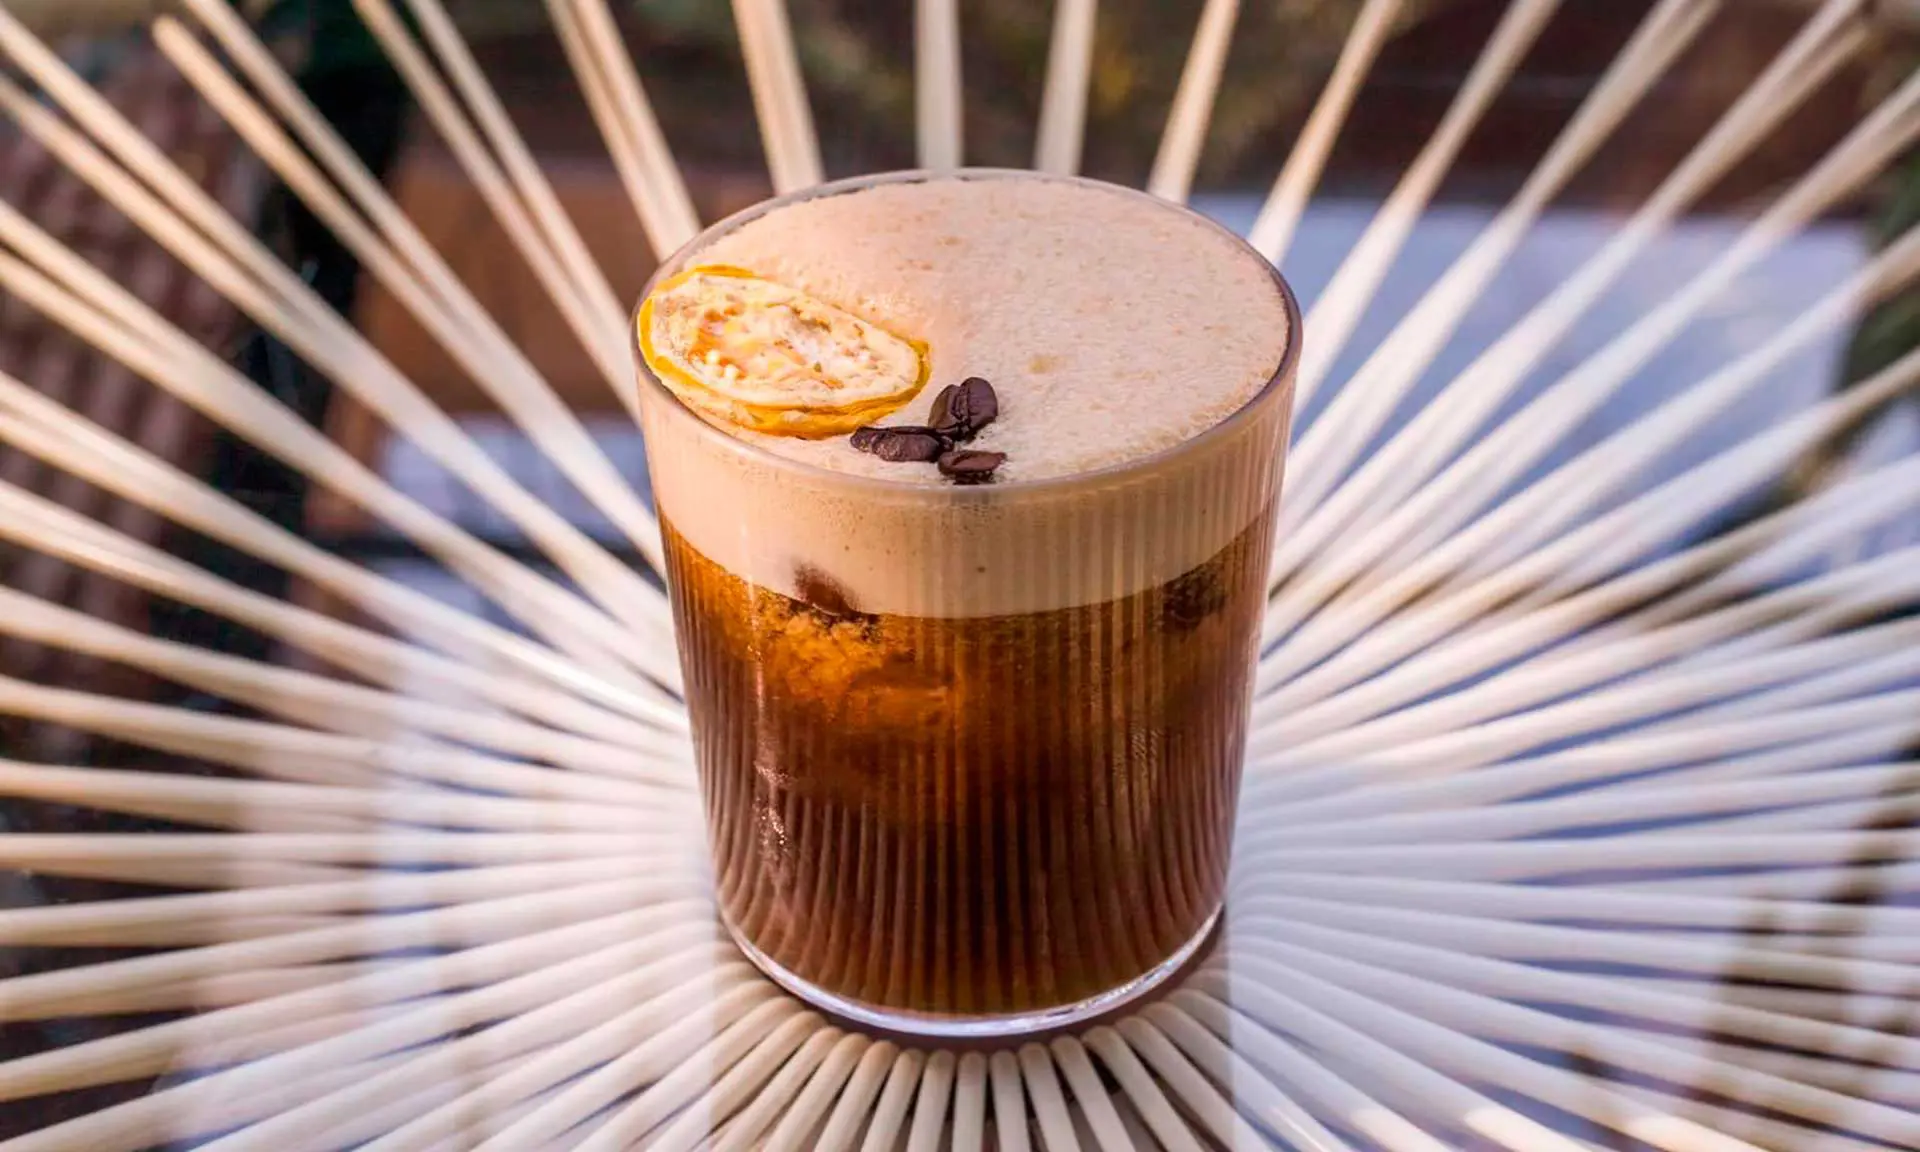
\includegraphics[width=5.5cm]{LOGO.png}
\tableofcontents\newpage}
\section{Setup Concurso}%%%%%%%%%%%%%%%%%%AYUDAMEMORIA%%%%%%%%%%%%%%%%
\subsection*{File setup}
\begin{code}
//tambien se pueden usar comas: {a, x, m, l}
touch {a..l}.in; tee {a..l}.cpp < tem.cpp
\end{code}
(agregar más)

\section{Directivas de concurso}
¿Ya consideraste todos los casos?

\begin{itemize}
\item Sin nadie lo lleva, es porque es dificil, espera a que alguien lo suba :p
\item Falta de un long long (WA) :c
\item const int N es incorrecta (WA, RTE)
\item Casos de n pequeña, especiales (RTE)
\item Division entre 0 (WA, RTE)
\item Acceso a una posicion no existente (RTE)
\item setprecision no correcto (WA)
\item Ciclo infinito, revisa esos while( true ) (TLE)
\item Reiniciar las variables, arreglos, estructuras sin son MUCHOS casos (WA)
\item mx/mn incorrectos (WA)
\item Enviar debugs (WA)
\item Uso de una variable que no es (WA)
\item Sigue intentando, el penalty es hasta que sea AC :p
\item long double, el double no sirve :'c
\item eps = 1e-9 es importante, sino NO va a jalar
\item Haz casos ptm!
\end{itemize}
\section{Template}
\cppfile{../Imprimibles/Standards/tem.cpp}
\end{document}
